\documentclass[11pt]{article}
\usepackage{graphicx} % Allows including images
\usepackage{booktabs} % Allows the use of \toprule, \midrule and \bottomrule in tables
\usepackage[belowskip=0pt,aboveskip=0pt]{caption}
\usepackage{amsmath}
\usepackage{pifont}
\usepackage{amsthm}
\usepackage{caption}
\usepackage[]{epstopdf}
\usepackage{braket}
%\usepackage{color}
\usepackage{mathtools}


\usepackage{listings}
\lstdefinestyle{mystyle}{
%    backgroundcolor=\color{backcolour},   
%    commentstyle=\color{codegreen},
%    keywordstyle=\color{magenta},
%    numberstyle=\tiny\color{codegray},
%    stringstyle=\color{codepurple},
    basicstyle=\footnotesize,
    breakatwhitespace=false,         
    breaklines=true,                 
    captionpos=b,                    
    keepspaces=true,                 
    numbers=left,                    
    numbersep=5pt,                  
    showspaces=false,                
    showstringspaces=false,
    showtabs=false,                  
    tabsize=2
}
 
\lstset{style=mystyle}


\usepackage{caption}

\usepackage{amsthm,amssymb,graphicx,graphicx,multirow,amsmath,cite}
\usepackage{float}
\usepackage{hyperref}
%\usepackage{minted} %Python Pygments
%\usepackage{listings}
\usepackage[usenames,dvipsnames]{color}
\usepackage{etoolbox}
\include{notation}
\oddsidemargin=0.15in
\evensidemargin=0.15in
\topmargin=-.5in
\textheight=9in
\textwidth=6.25in
%\bootrue{Advanced}

\newtheorem{lemma}{Lemma}{}
  \newtheorem{thm}{Theorem}
  \newtheorem{theorem}{Theorem}
  \newtheorem{prop}{Proposition}
  \newtheorem{cor}[thm]{Corollary}
  \newtheorem{defi}[thm]{Definition}
  \newtheorem{definition}[thm]{Definition}
  
  %% USE THESE IN YOUR TEX CODE.
\def\E{\mathbb{E}} % For Expectation
\def\P{\mathbb{P}} % for probabiltiy
\def\EE{\mathbb{E}^{!o}} % For Palm expectation
\def\ie{{\em i.e.}} 
\def\eg{{\em e.g.}}
\def\V{\operatorname{Var}}
\def\L{\mathcal{L}} % For Laplace transform
\def\i{\mathbf{1}} % Indicator random variable
\def\l{\ell}% For path loss moel


\definecolor{mygreen}{rgb}{0,0.6,0}
\definecolor{mygray}{rgb}{0.5,0.5,0.5}
\definecolor{mymauve}{rgb}{0.58,0,0.82}

\lstset{ %
  backgroundcolor=\color{white},   % choose the background color
  basicstyle=\footnotesize,        % size of fonts used for the code
  breaklines=true,                 % automatic line breaking only at whitespace
  captionpos=b,                    % sets the caption-position to bottom
  commentstyle=\color{mygreen},    % comment style
  escapeinside={\%*}{*)},          % if you want to add LaTeX within your code
  keywordstyle=\color{blue},       % keyword style
  stringstyle=\color{mymauve},     % string literal style
}



\begin{document}
%--------------
%% preamble.tex
%% this should be included with a command like
%% %--------------
%% preamble.tex
%% this should be included with a command like
%% %--------------
%% preamble.tex
%% this should be included with a command like
%% \input{preamble.tex}
%% \lecture{1}{September 4, 1996 }{Daniel A. Spielman}{name
%%  of poor scribe}

\hbadness=10000
\vbadness=10000

\setlength{\oddsidemargin}{.25in}
\setlength{\evensidemargin}{.25in}
\setlength{\textwidth}{6in}
\setlength{\topmargin}{-0.4in}
\setlength{\textheight}{8.5in}

\newcommand{\handout}[5]{
   \renewcommand{\thepage}{#1-\arabic{page}}
   \noindent
   \begin{center}
   \framebox{
      \vbox{
    \hbox to 5.78in { {\b APPM7440: Radial Basis Functions - Finite Differences

 }
     	 \hfill #2 }
       \vspace{4mm}
       \hbox to 5.78in { {\Large \hfill #5  \hfill} }
       \vspace{2mm}
       \hbox to 5.78in { {\it #3 \hfill #4} }
      }
   }
   \end{center}
   \vspace*{4mm}
}

\newcommand{\lecture}[4]{\handout{#1}{#2}{ #3}{Scribe: #4}{ Lecture #1}}
\newcommand{\assignment}[5]{\handout{#1}{#2}{ #3}{Author: #4(#5)}{ Assignment #1}}
\newcommand{\labreport}[5]{\handout{#1}{#2}{ #3}{Author: #4(#5)}{ Lab Report #1}}
%% \lecture{1}{September 4, 1996 }{Daniel A. Spielman}{name
%%  of poor scribe}

\hbadness=10000
\vbadness=10000

\setlength{\oddsidemargin}{.25in}
\setlength{\evensidemargin}{.25in}
\setlength{\textwidth}{6in}
\setlength{\topmargin}{-0.4in}
\setlength{\textheight}{8.5in}

\newcommand{\handout}[5]{
   \renewcommand{\thepage}{#1-\arabic{page}}
   \noindent
   \begin{center}
   \framebox{
      \vbox{
    \hbox to 5.78in { {\b APPM7440: Radial Basis Functions - Finite Differences

 }
     	 \hfill #2 }
       \vspace{4mm}
       \hbox to 5.78in { {\Large \hfill #5  \hfill} }
       \vspace{2mm}
       \hbox to 5.78in { {\it #3 \hfill #4} }
      }
   }
   \end{center}
   \vspace*{4mm}
}

\newcommand{\lecture}[4]{\handout{#1}{#2}{ #3}{Scribe: #4}{ Lecture #1}}
\newcommand{\assignment}[5]{\handout{#1}{#2}{ #3}{Author: #4(#5)}{ Assignment #1}}
\newcommand{\labreport}[5]{\handout{#1}{#2}{ #3}{Author: #4(#5)}{ Lab Report #1}}
%% \lecture{1}{September 4, 1996 }{Daniel A. Spielman}{name
%%  of poor scribe}

\hbadness=10000
\vbadness=10000

\setlength{\oddsidemargin}{.25in}
\setlength{\evensidemargin}{.25in}
\setlength{\textwidth}{6in}
\setlength{\topmargin}{-0.4in}
\setlength{\textheight}{8.5in}

\newcommand{\handout}[5]{
   \renewcommand{\thepage}{#1-\arabic{page}}
   \noindent
   \begin{center}
   \framebox{
      \vbox{
    \hbox to 5.78in { {\b APPM7440: Radial Basis Functions - Finite Differences

 }
     	 \hfill #2 }
       \vspace{4mm}
       \hbox to 5.78in { {\Large \hfill #5  \hfill} }
       \vspace{2mm}
       \hbox to 5.78in { {\it #3 \hfill #4} }
      }
   }
   \end{center}
   \vspace*{4mm}
}

\newcommand{\lecture}[4]{\handout{#1}{#2}{ #3}{Scribe: #4}{ Lecture #1}}
\newcommand{\assignment}[5]{\handout{#1}{#2}{ #3}{Author: #4(#5)}{ Assignment #1}}
\newcommand{\labreport}[5]{\handout{#1}{#2}{ #3}{Author: #4(#5)}{ Lab Report #1}}
\labreport{3}{April 30, 2015}{Homework 3}{Prasanth Prahladan}{100817764}

\section{GA-RBF Standard Double Precision Implementation}


\begin{figure}[h!]
\centering
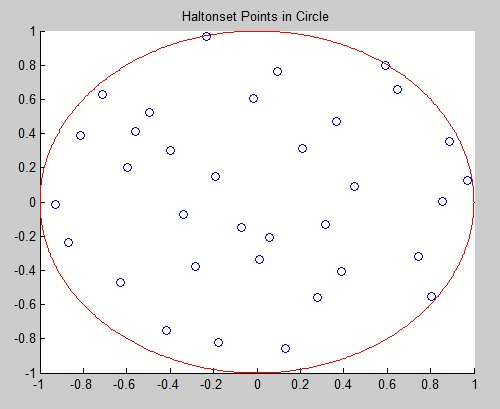
\includegraphics[scale=0.4]{hw3_halton.jpg}\\
\caption{Haltonset node distribution in Circular Disc}
\label{fig:haltonSet}
\end{figure}



\begin{figure}[h!]
\centering
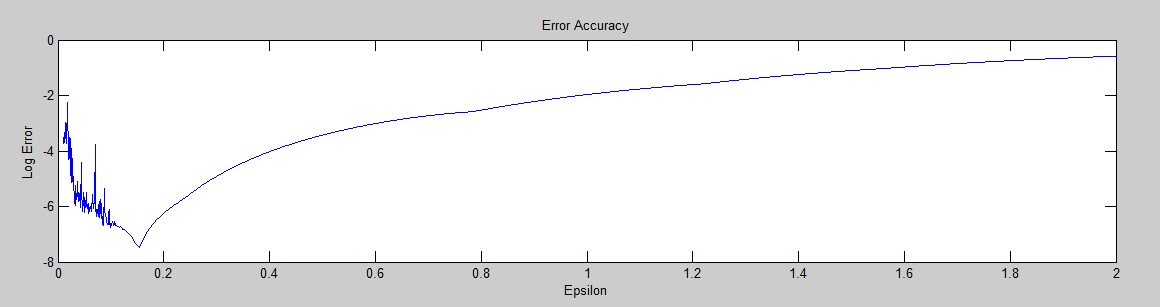
\includegraphics[scale=0.5]{hw3_error.jpg}\\
\caption{Log10(Error) variation with $\epsilon$}
\label{fig:logError}
\end{figure}



\begin{figure}[h!]
\centering
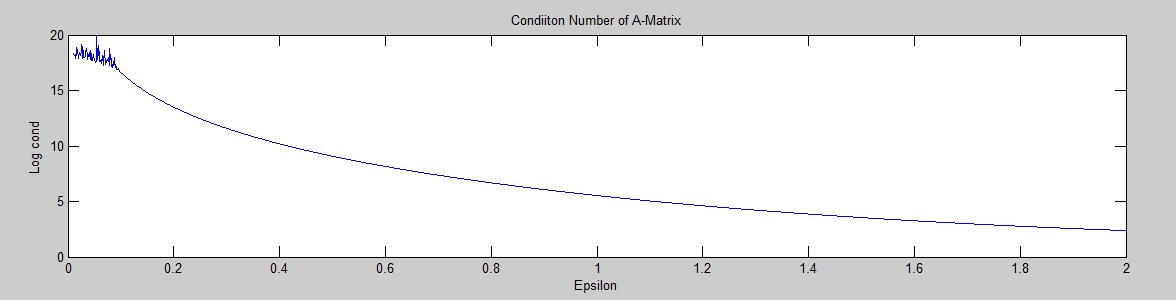
\includegraphics[scale=0.5]{hw3_cond.jpg}\\
\caption{Variation of Condition Number of A matrix with $\epsilon$}
\label{fig:condNumber}
\end{figure}



\subsection{Matlab Implementation}

\begin{lstlisting}[language=octave]
% APPM 7440: HW#3
% Question 1: Double Precision Arithmetic
% RBF - DIRECT 
% ========================================================================
close all
clear all
clc

N = 42;         % Total sample points needed : Always Ensure EVEN!!

%%
% GENERATE POINTS WITHIN UNIT CIRCLE - can be done as a function.

% plot unit circle
theta = 0:0.01:2*pi;
circx = cos(theta);
circy = sin(theta);
fig1 = figure(1)
plot(circx,circy,'r')
hold on
%%
% Generate Uniformly Random distributed points in Unit Disc

rndTheta = 2*pi*rand(N,1);
rndRad1 = sqrt(rand(N,1));
x1 = rndRad1.*cos(rndTheta);
y1 = rndRad1.*sin(rndTheta);
scatter(x1,y1)
title('Uniformly Distributed Points in Unit Disc')
hold off

% xvecs = [x1' y1']; % Nx2 matrix.

%%
% Generate Random points using HaltonSet

rng default
p = haltonset(2,'Skip',1e3,'Leap', 1e2);
p = scramble(p,'RR2');      % Reverse radix scrambling
X0 = net(p,N);
X0 = -1*ones(size(X0)) + 2*X0;
R = sqrt(X0(:,1).^2 + X0(:,2).^2);
inds = find((R<=1));
x2 = X0(inds,1);
y2 = X0(inds,2);

% -----------------------------------
fig2 = figure(2)
scatter(x2,y2,'b')
title('Haltonset Points in Circle')
hold on
plot(circx,circy,'r')
hold off


%%
% Choose the data-set you want from ABOVE
% (x2,y2): Haltonset ; (x1,y1): RandomNumbers

% #COLUMNS = # Dimensions of the Spatial Vectors
% #ROWS = # Data Points

x0 = x2;
y0 = y2;

% x = floor(10*rand(1,5));
% y = floor(10*rand(1,5));

% Divide Data Points into GRID(TRAIN) and TEST LOCATIONS
x_trn = x0(1:N/2)';
y_trn = y0(1:N/2)';
Z_trn = [x_trn; y_trn]';   
size(Z_trn)

x_tst = x0(N/2+1:end)';
y_tst = y0(N/2+1:end)';
Z_tst = [x_tst; y_tst]';


%%
% Checking for errors when the Test Data is same as Training Data
% Z_tst = Z_trn(2:4,:);
 Z_tst = Z_tst;
%%  MAIN SECTION: Iterating over SHAPE PARAMTER

% Evaluate Test Function : Train Data
fvals_trn = evalTestFunction(Z_trn);
size(fvals_trn)

% Evaluate Test Function : Testing Data
fvals_tst = evalTestFunction(Z_tst);
size(fvals_tst)

Epsilon = 0.01:0.001:2;
% ------------------------------------------------------------
% Epsilon = ones(size(Epsilon)); % Test Case for Accuracy
% When eps = 1, the Reciprocal Condition-Number should be closer to 1.
% ------------------------------------------------------------
error = zeros(size(Epsilon));
Condition = zeros(size(Epsilon));
Lambda = zeros(size(Epsilon));
Fvals = zeros(size(Epsilon));

% ----------------------------------------------------------------
for count = 1:length(Epsilon)
% Compute Lambda
% --------------------------
% fprintf('Z_trn Dimensions \n')
% size(Z_trn)
epsilon = Epsilon(count);
A_trn = getRBFmatrix(Z_trn,epsilon,'GA');
% fprintf('Size A_trn \n')
% size(A_trn)
lambda = A_trn\fvals_trn;

% Evaluate the function at 
feval_tst = evalRBFinterpolation(Z_tst,Z_trn,lambda, epsilon,'GA');

fprintf('Size feval_tst \t')
size(feval_tst)
fprintf('Size fvals_tst \t')
size(fvals_tst)

% Compute the parameters to plot.
Condition(count) = cond(A_trn);
error(count) = max(abs(feval_tst - fvals_tst));

% unnecessary params
Lambda(count) = max(abs(lambda));
Fvals(count) = max(abs(fvals_trn));

% break         % Used for Testing!

end

count
fig4 = figure(4)
subplot(2,1,1)
% plot(Epsilon, Lambda)
plot(log10(Lambda))        % TEST
xlabel('Epsilon')
ylabel('Log Max Lambda')
subplot(2,1,2)
% plot(Epsilon, Fvals)
plot(Fvals)         % TEST
xlabel('Epsilon')
ylabel('Fvals')

fig5 = figure(5)
subplot(2,1,1)
plot(Epsilon, log10(error))
% plot(error)         % TEST
title('Error Accuracy')
xlabel('Epsilon')
ylabel('Log Error')
subplot(2,1,2)
plot(Epsilon, log10(Condition))
% plot(Condition)     % TEST
title('Condiiton Number of A-Matrix')
xlabel('Epsilon')
ylabel('Log cond')



% ======================================================================
% ======================================================================
% APPM 7440: HW#3
% Question 1: Double Precision Arithmetic

function A = getRBFmatrix(Z,epsilon, RBFtype)
%{
Z           : Data point vectors
epsilon     : Shape Parameter
RBFtype     : Type of RBF used
%}

[rows,cols] = size(Z);
if cols ==1
    X = Z(:,1)'; % row vector
    [Ggrid, Gvar] = meshgrid(X,X);
    dX = Gvar - Ggrid;
    R2 = dX.^2;
    
elseif cols == 2 % 2-dimensional dataset
    % row-vectors
    X = Z(:,1)';
    Y = Z(:,2)';
    
    % grid ------------------------
    [gx, gy] = meshgrid(X,Y);
    GY = gy';
    GX = gx;
    
    % Compute RBF
    dX = GX' - GX;
    dY = GY' - GY;
    R2 = dX.^2 + dY.^2
    
else
    prinft('ERROR: Does not support greater than 2 Dimensions!')
end

% Create RBF Matrix
% ---------------------------
ONE = ones(size(R2));
switch RBFtype
    case 'GA' % RBF: Gaussian
        fprintf('Gaussian \n')
        A = exp(-(epsilon^2)*R2)
        
    case 'IMQ' % RBF: Inverse Multiquadric
        fprintf('Inverse Multiquadric \n')
        A = 1./(ONE + (epsilon^2)*R2).^(1/2);
        
    case 'IQ' % RBF: Inverse Quadratic
        fprintf('Inverse Quadratic \n')
        A = 1./(ONE + (epsilon^2)*R2);
        
    otherwise % RBF: Multi-Quadrics
        fprintf('Multi-Quadrics \n')
        A = (ONE + (epsilon^2)*R2).^(1/2);
        
end
return

% ===========================================================
% ===========================================================
% APPM 7440: HW#3
% Question 1: Double Precision Arithmetic

function feval = evalRBFinterpolation(Z_data, Z_grid,lambda, epsilon, RBFtype)
%{
Z_data      : Data point vectors
Z_grid      : Grid point vectors
lambda      : RBF Interpolation Coefficients
epsilon     : Shape Parameter
RBFtype     : Type of RBF used
%}

% MQ-RBF/ GA-RBF methodology for function interpolation
% and computing error.
% --------------------------
% Compute as a function of shape-parameter
% --------------------------
% meshgrid and ndgrid to compute the A matrix
% --------------------------

[r,c] = size(Z_data);
if c ==1 % 1-Dimensional Data
    X_data = Z_data(:,1)';
    X_grid = Z_grid(:,1)';
    
    G = ndgrid(X_grid, X_data);
    GridX = G';
    DataX = ndgrid(X_data, X_grid);
    
    dX = DataX - GridX;
    
    R2 = dX.^2;
    
elseif c == 2 % 2-dimensional dataset
    X_data = Z_data(:,1)'
    Y_data = Z_data(:,2)'
       
    X_grid = Z_grid(:,1)'
    Y_grid = Z_grid(:,2)'

    % ==================================
    G = ndgrid(X_grid, X_data);
    GridX = G'
    DataX = ndgrid(X_data, X_grid)
    
   
    G = ndgrid(Y_grid, Y_data);
    GridY = G'
    DataY = ndgrid(Y_data, Y_grid)
    
    % ============================
    % Compute RBF
    
    dX = DataX - GridX;
    dY = DataY - GridY;
    R2 = dX.^2 + dY.^2;
    
else
    fprintf('>2-Dimensions NOT supported!')
end

% Create RBF Matrix
% ---------------------------
ONE = ones(size(R2));
switch RBFtype
    case 'GA' % RBF: Gaussian
        fprintf('Gaussian \n')
        A = exp(-(epsilon^2)*R2)
        
    case 'IMQ' % RBF: Inverse Multiquadric
        fprintf('Inverse Multiquadric \n')
        A = 1./(ONE + epsilon^2*R2).^(1/2);
        
    case 'IQ' % RBF: Inverse Quadratic
        fprintf('Inverse Quadratic \n')
        A = 1./(ONE + epsilon^2*R2);
        
    otherwise % RBF: Multi-Quadrics
        fprintf('Multi-Quadrics \n')
        A = (ONE + epsilon^2*R2).^(1/2);
end

feval = A*lambda

return
\end{lstlisting}

\section{GA-RBF: Variable Precision Arithmetic}


\subsection{Matlab Implementation}
\begin{lstlisting}[language=octave]
% APPM 7440: HW#3
% Question 2: VARIABLE Precision Arithmetic
% RBF - DIRECT
% ========================================================================
close all
clear all
clc

N = 42;         % Total sample points needed : Always Ensure EVEN!!

%%
% GENERATE POINTS WITHIN UNIT CIRCLE - can be done as a function.

% plot unit circle
theta = 0:0.01:2*pi;
circx = cos(theta);
circy = sin(theta);

fig1 = figure(1)
plot(circx,circy,'r')

%%
% Generate Random points using HaltonSet

rng default
p = haltonset(2,'Skip',1e3,'Leap', 1e2);
p = scramble(p,'RR2');      % Reverse radix scrambling
X0 = net(p,N);
X0 = -1*ones(size(X0)) + 2*X0;
R = sqrt(X0(:,1).^2 + X0(:,2).^2);
inds = find((R<=1));
x2 = X0(inds,1);
y2 = X0(inds,2);

% -----------------------------------
fig2 = figure(2)
% subplot(2,1,1)
scatter(x2,y2,'b')
title('Haltonset Points in Circle')
hold on
plot(circx,circy,'r')
hold off

%%
% Choose the data-set you want from ABOVE
% (x2,y2): Haltonset ; (x1,y1): RandomNumbers

% #COLUMNS = # Dimensions of the Spatial Vectors
% #ROWS = # Data Points

x0 = sym(x2);
y0 = sym(y2);

% Divide Data Points into GRID(TRAIN) and TEST LOCATIONS
% Grid-Training Data
x_trn = x0(1:N/2)';
y_trn = y0(1:N/2)';
Z_trn = [x_trn; y_trn]';
Z_trn = sym(Z_trn);

% Testing Data
x_tst = x0(N/2+1:end)';
y_tst = y0(N/2+1:end)';
Z_tst = [x_tst; y_tst]';
Z_tst = sym(Z_tst);

%%  MAIN SECTION: Iterating over SHAPE PARAMTER

% Describe Test Function
testFunc = @(Z)( sym(59) ./ sym(67 + ( sym(Z(:,1)) + 1/sym(7) ).^2 + ( sym(Z(:,2)) - 1/sym(11) ).^2 ) );

% Evaluate Test Function : Train Data
fvals_trn = testFunc(Z_trn);
fvals_trn = sym(fvals_trn);
% fprintf('\nSize fvals_trn \t'); size(fvals_trn)

% Evaluate Test Function : Testing Data
fvals_tst = testFunc(Z_tst);
fvals_tst = sym(fvals_tst);
% fprintf('\nSize fvals_tst \t'); size(fvals_tst)

% ===============================================
% Evlauation for Training Data

X_trn = sym(Z_trn(:,1));
Y_trn = sym(Z_trn(:,2));

% grid ------------------------
[gx, gy] = meshgrid(X_trn,Y_trn);
GY = sym(gy');
GX = sym(gx);

% Compute RBF
dX = sym(GX' - GX);
dY = sym(GY' - GY);
R2Trn = sym(dX.^2 + dY.^2);
rTrn = sym(sqrt(R2Trn));
% fprintf('\nSize rTrn \t');size(rTrn)

% ========================================
% Computations for Testing Data
X_tst = sym(Z_tst(:,1));
Y_tst = sym(Z_tst(:,2));

[nodeX,gridX] = ndgrid(X_tst,X_trn);
[nodeY,gridY] = ndgrid(Y_tst,Y_trn);

R2tst = (sym(nodeX)-sym(gridX)).^2 + (sym(nodeY) - sym(gridY)).^2;
rTst = sqrt(sym(R2tst));
% fprintf('\nSize rTst \t');size(rTst)
% ===============================================
% ------------------------------------------------------------
% Epsilon = ones(size(Epsilon)); % Test Case for Accuracy
% When eps = 1, the Reciprocal Condition-Number should be closer to 1.
% ------------------------------------------------------------
Epsilon = 0.001:0.001:1;

error = zeros(size(Epsilon));
Condition = zeros(size(Epsilon));
Lambda = zeros(size(Epsilon));
Fvals = zeros(size(Epsilon));
% ===============================================
% Description of RBF Function
fi = @(r,ep)(exp(-(ep*r).^2)); % GA-RBF

ACC = 2^10; % VPA Precision Digits
profile ON
% ----------------------------------------------------------------
for count = 1:length(Epsilon)
% count = 1;
    
    epsilon = Epsilon(count);
    fprintf('epsilon \t %f \n',epsilon)
    epsilon = sym(epsilon);
    
    % Compute Lambda
    % --------------------------
    A_trn = fi(rTrn,epsilon);
    
    nmA_trn = vpa(A_trn,ACC);
%     fprintf('\nSize A_trn \t');size(A_trn)
    
%     invA_trn = vpa(inv(A_trn),ACC);
%     fprintf('\nSize invA_trn \t');size(invA_trn)    
    
%     fprintf('\nSize fvals_trn \t');size(fvals_trn)
    
    lambda = nmA_trn\fvals_trn;
    lambda = sym(lambda);
%     fprintf('\n Size lambda \t');size(lambda)
    
    % Evaluate the function at Test Points
    % --------------------------
    A_tst = fi(rTst,epsilon);
%     A_tst = sym(A_tst);
%     fprintf('\nSize A_tst \t');size(A_tst)
    
    feval_tst = A_tst*lambda;
    feval_tst = sym(feval_tst);
%     fprintf('\nSize feval_tst \t');size(feval_tst)
    
    % Compute the parameters to plot.
    % --------------------------
    Condition(count) = cond(nmA_trn);
    err = vpa(feval_tst - fvals_tst, ACC);
    error(count) = max(abs(err));
    
    % unnecessary params
    Lambda(count) = max(abs(vpa(lambda,ACC)));
    Fvals(count) = max(abs(vpa(fvals_trn,ACC)));
    
end

profile VIEWER

count


fig4 = figure(4)
subplot(2,1,1)
% plot(Epsilon, Lambda)
plot(log10(Lambda))        % TEST
xlabel('Epsilon')
ylabel('Log Max Lambda')
subplot(2,1,2)
% plot(Epsilon, Fvals)
plot(Fvals)         % TEST
xlabel('Epsilon')
ylabel('Fvals')

fig5 = figure(5)
subplot(2,1,1)
plot(Epsilon, log10(error))
% plot(error)         % TEST
title('Error Accuracy')
xlabel('Epsilon')
ylabel('Log Error')
subplot(2,1,2)
plot(Epsilon, log10(Condition))
% plot(Condition)     % TEST
title('Condiiton Number of A-Matrix')
xlabel('Epsilon')
ylabel('Log cond')
\end{lstlisting}

\subsection{Plots and Results}

\begin{figure}[h!]
\centering

\includegraphics[scale=0.5]{profileTime.jpg}\\
\caption{Profile Times}
\label{fig:profileTime}
\end{figure}



\begin{figure}[h!]
\centering
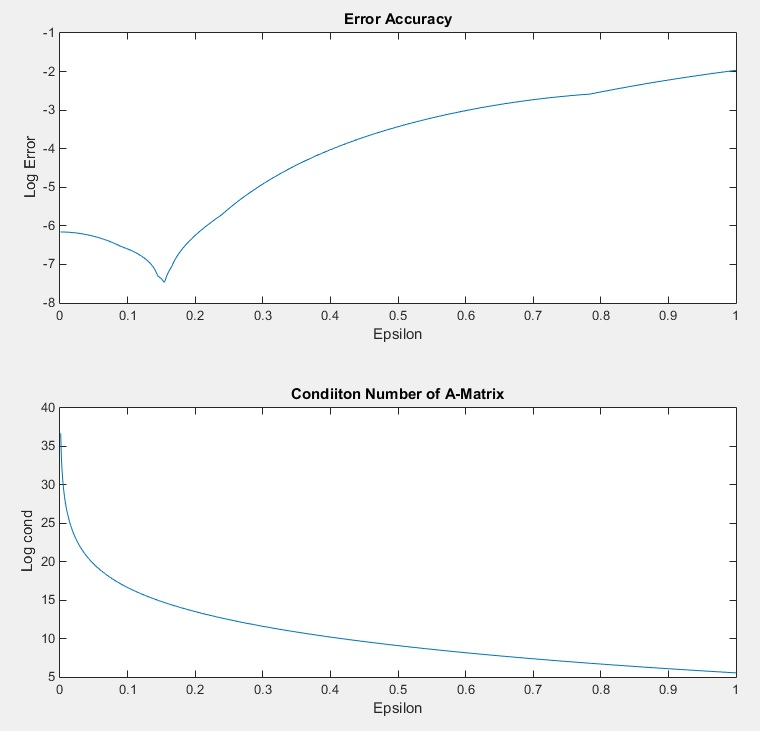
\includegraphics[scale=0.7]{vpaError.jpg}\\
\caption{log10(Error) and Condition Number Plots}
\label{fig:vpaError}
\end{figure}


\end{document}



